\documentclass[12pt,a4paper]{ctexart}
\usepackage{ctex}
\usepackage{emptypage} 
\usepackage{fancyhdr}
\usepackage{amsmath,amsfonts,amssymb,mathtools}
\usepackage{graphicx}
\usepackage{mathptmx}
\usepackage{booktabs}
\usepackage[labelfont=bf]{caption}
\usepackage{indentfirst}
\usepackage{caption}
\usepackage{enumitem}
\usepackage[marginal]{footmisc}
\usepackage{subfigure}
\usepackage{fontspec}
\usepackage{geometry}
\usepackage{setspace}
\usepackage{listings}
\usepackage{xcolor}
\usepackage{float}
\newgeometry{left=3cm,top=2.5cm,bottom=2.5cm,right=3cm}
\setmainfont{Times New Roman}
\setCJKmainfont[BoldFont=SimHei,ItalicFont=KaiTi]{SimSun}

\lstset{
	backgroundcolor=\color{green!10!blue!15},%代码块背景色
	rulesepcolor= \color{red!40!blue!100}, %代码块边框颜色
	breaklines=true,  %代码过长则换行
	breakatwhitespace=false,
	numbers=left, %行号在左侧显示
	numberstyle= \small,%行号字体
	keywordstyle= \color{blue},%关键字颜色
	commentstyle=\color{gray}, %注释颜色
	frame=shadowbox%用方框框住代码块
}

\renewcommand{\baselinestretch}{1.5}%可加可不加,控制行间距

\title{\textbf{对现有自动驾驶相关技术发展与分析\\及对自动驾驶的未来展望和思考}}%标题

\author{
\\
\Large{麻超 \quad 201300066}
\\[6pt]
{ \large \textit{南京大学人工智能学院}}\\[2pt]
}

\date{}
\newcommand{\supercite}[1]{\textsuperscript{\cite{#1}}}

\begin{document}
\maketitle
\setcounter{page}{1}
\textbf{摘要} \quad {随着人工智能技术的发展势头迅猛,自动驾驶逐渐进入公众视野,国内外许多车企巨头竞相开发自动驾驶汽车,又有许多的新型科技公司崛起,妄图在自动驾驶的领域分一杯羹。随着科技的逐渐进步,自动驾驶离我们貌似已经不再遥远。本文拟从$Tesla$,$Horizon$ $Robotics$,$Momenta$三家类型不一的公司公司入手,浅析其产品的进度与当前自动驾驶相关评估系统与技术发展,并对未来的自动驾驶做一个展望。} \\

\textbf{关键词}\quad {自动驾驶;智能化评估;传感器识别;高精地图}
\\[60pt]

\section*{引言}

近三十年来,移动机器人除了在宇宙探测、海洋开发和原子能等领域有广泛的应用以外,在工厂自动化、建筑、采矿、排险、军事、服务、农业等方面也有广泛的应用前景。移动机器人按照应用领域分可以分为工业机器人、探索机器人、服务机器人、军事机器人等,而按照其移动机构,则可以划分为轮式、履带式、足式、混合式、特殊式等类型机器人$^{[1]}$。其中,足式机器人和轮式机器人、履带式机器人又是应用最广泛的三者。机器人运动系统是移动设计的本质特征,它不仅取决于工作空间,还取决于机动性、可控性、地形条件、效率和稳定性等技术指标,每个系统都有自己的优点和缺点$^{[2]}$。足式机器人与轮式机器人技术标准的详细比较如表格所示。从表格可以看出,足式机器人在过去几十年中不断发展,现在它比轮式机器人车辆更具优势。
\begin{table}[ht]
	\centering
	\caption{轮式机器人与足式机器人比较}\label{}
	\tabcolsep 15pt
	\begin{tabular}{c|c|c}
		\hline
		技术标准           & 轮式机器人 & 足式机器人 \\
		\hline
		机动性             & $\times$   & $\surd$    \\
		横向能力           & $\times$   & $\surd$    \\
		可控性             & $\surd$    & $\times$   \\
		地形土地           & $\times$   & $\surd$    \\
		效率               & $\times$   & $\surd$    \\
		稳定               & $\surd$    & $\times$   \\
		成本效益           & $\surd$    & $\times$   \\
		越过障碍物导航能力 & $\times$   & $\surd$    \\
		\hline
	\end{tabular}
\end{table}

足运动的优势取决于姿势、足的数量和足的功能。轮式和履带式机器人虽然可以在平面地形上工作,但大多数不能在地形复杂、环境复杂和危险的环境下工作。足式机器人更有可能在像人类或者动物一样\supercite{3},在地球的各个表面的不同地形上漫游。动物用它们的腿在不同的地形中快速移动,具有出色的运动姿态和敏捷性。大多数情况下,它们会根据环境条件提高速度和效率。从稳定性和高效的步态来看,四足机器人是所有与移动性和运动稳定性相关的足式机器人中的最佳选择。与两条或六条足相比,四足机器人易于控制、设计和维护。为了实现像牛、狗、猎豹那样的实时速度和自然运动,需要开发控制系统和四足机器人的动态步态生成。
\section{国外的四足机器人发展}
\subsection{1900年代早期的四足机器人}
在1900年代初期,许多科学家和研究人员正致力于研究四足机器人的足机构。切比雪夫于1870年研制出第一个行走机构,主要是在四杆机构的基础上将旋转运动转化为匀速平移运动,如图1所示。该设备只能在平坦的地形上动态行走,没有独立的腿部运动。后来,这种机制被合并到两台机器 MELWALK 和 DANTE \supercite{4}中。
\begin{figure}[H]
	\centering
	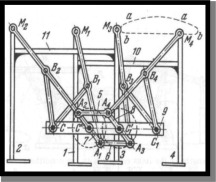
\includegraphics[height=4.5cm]{IMG_01.jpg}
	\caption{切比雪夫的行走机构模型}
\end{figure}
后来,Raibert研制出另一种步行结构,称为“机械马”\supercite{5},如图所示,使用不同类型的连杆和曲柄通过骑手踏板将动力传递给机器。Hutchinson于1940年在英国进行了最早的专门尝试建造具有独立控制腿的机车机器\supercite{6},如图所示。这是一个四足模型,高约60厘米,其八个关节由柔性电缆控制,而柔性电缆又由操作者的两只脚和双手控制。后来,这个概念被通用电气在1960年代用于MOSHER/WALKING TRUCK,如图。
\begin{figure}[H]
	\centering
	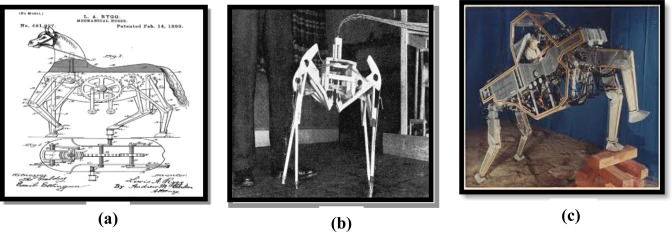
\includegraphics[height=4.5cm]{IMG_02.jpg}
	\caption{机械马的结构和实现}
\end{figure}
\subsection{1900年代中期的四足机器人}
美国第一个自主四足机器人于 1960 年代在南加州大学建造。它被命名为“phony pony”\supercite{7}.该机器人的每条腿都有两个相同的旋转关节,具有电动驱动并能够产生多种步态模式像小跑一样,走路包括以缓慢的速度爬行。它还能够保持静止的直立稳定步态,因为每只脚都基于倒T形或骨盆结构,可在正面提供稳定性。

1976年,Hirose和Kato在四足动物的发展中带来了一个重要的里程碑,特别是受到长腿蜘蛛的启发,研制出蜘蛛状四足机器人\supercite{8}。蜘蛛状四足机器人KUMO-1重14kg,长1.5m。每条腿都有一个驱动电机和一个离合器来产生行走运动。1980年代初期,机器人领域发生了一场革命,由Raibert和其在MIT的同事共同完成,他们共同做了一个可以实现类似于单腿袋鼠一样跳跃和奔跑的机器人\supercite{9}。
\subsection{1990年代的四足机器人}
独足平衡和动力学专利原理不仅超越了各种足系统,而且远远超越了任何生物足机器人。它实际上是对四足机器人运动稳定性的控制。Hirose的TITAN 系列\supercite{10}是四足机器人发展中最杰出的成就。首先,他开发了 TITAN-III 四足机器人,其中一个三维受电弓机构结合了一个腿机构,如图3(a)所示。这是世界上第一台攀爬机器人配备智能程序、脚趾触觉传感器和姿态传感器。TITAN-IV 于1986年开发,具有额外的功能,例如它可以通过逐渐增加速度将爬行步行转换为小跑,如图3(b)所示。同样,TITAN-V 和 TITAN-VI 开发用于其他测试目的,如重量、机构、动态行走等。行走四足机器人TITAN-VII\supercite{11}主要用于辅助在陡坡上的施工作业,如移动脚手架,如图3(c)所示。其中,TITAN-VIII\supercite{12}是最受欢迎的工作四足机器人。考虑到重力解耦驱动,它设计有一种新的系留驱动机制(GDA),腿长400m,重量40kg,如图4(a)所示。
\begin{figure}[H]
	\centering
	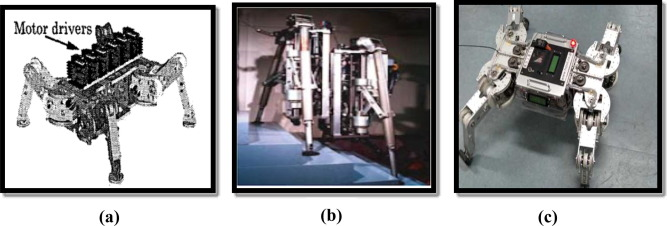
\includegraphics[height=4.5cm]{IMG_03.jpg}
	\caption{TITAN系列机器人}
\end{figure}

之后的TITAN系列机器人也被用于不同的领域,TITAN-IX用于人道主义排雷任务,如图4(b)所示。TITAN-XI\supercite{13]的性能与 TITAN-VII 相同,但在陡坡上具有钻孔等额外功能,如图4(c)所示。700公斤重的TITAN-XI内置有液压执行器、板载计算机。TITAN-XII\supercite{14}四足机器人可以通过外部计算机和微控制器精确地越过巨大的障碍物以及拥有1.5m/s的速度。
\begin{figure}[H]
	\centering
	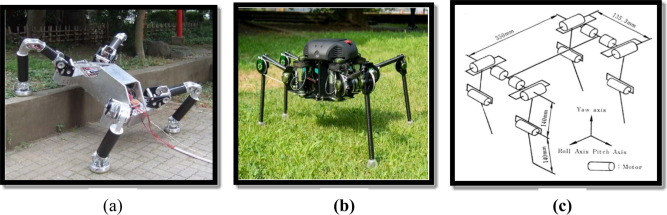
\includegraphics[height=4.5cm]{IMG_04.jpg}
	\caption{TITAN系列机器人-2}
\end{figure}
TITAN系列最新的行走四足机器人是TITAN XIII\supercite{15},它是一种伸展型四足机器人,TITAN XIII可以以1.38m/s的速度高速行走,并由电池供电。

1999年,SCOUT-I 和 II \supercite{16}\supercite{17}麦吉尔大学的Buchler和Robert设计了两款SCOUT-I 和 II,如图所示。在SCOUT-I中,每条腿只有一个驱动自由度,RC-Servomotor控制臀部运动。SCOUT-II是SCOUT-I的更大版本,其使用工作模型进行爬楼梯模拟以探索动态步态。瑞典皇家理工学院于1998年开发了仿生四足机器人WRAP1\supercite{18},用于研究崎岖地形中的静态和动态运动。WRAP1重约60公斤,共有12个ROF。由专用的6个控制器局域网(CAN)总线很好地控制的自由度。
\begin{figure}[H]
	\centering
	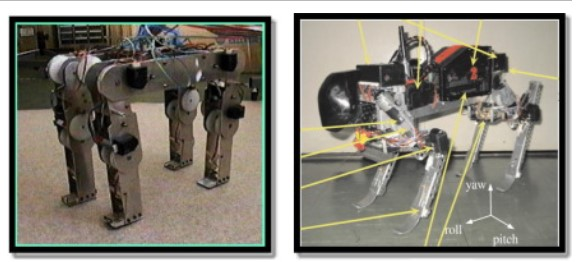
\includegraphics[height=4.5cm]{IMG_05.jpg}
	\caption{SCOUT-I和SCOUT-II}
\end{figure}
\subsection{21世纪初的四足机器人}
SILO4是西班牙工业自动化研究所(CSIC)于1999年设计的四足步行机器人\supercite{19},如图11(b)所示. 设计师的主要目标是专注于运动生成、地形适应和稳定性。它共有 12 个自由度,并通过电驱动模仿昆虫的腿。在实验上,它用于开发教育机器人和不同研究人员的需求。

成均馆大学机械工程学院为工业公用事业设计了用于墙壁检查的多功能机器人-III(MRWALLSPECT-III),其具有更好的地形适应性,如步入式飞机,使用吸盘爬上带有凸角的墙壁,作为如图12 (b)\supercite{20}所示。活动关节由三齿轮直流电机精确驱动。它有两个控制器;一种是使用 Pentium-III 嵌入的,另一种是 Real Time-Linux (RT-Linux)。在MRWALLSPECT-III之后不久,他们又于2007年开发了另一款狗型四足步行机器人,命名为AiDAN-I,随后于2013年开发了AiDAN-III,如图12(c)和图13(一)\supercite{21}\supercite{22}。机器人的每个肢体都有3个自由度和一个被动关节,它有一个中央控制器和16个子控制器,每个控制器都嵌入了 CAN配置并由RT-Linux操作。
\begin{figure}[H]
	\centering
	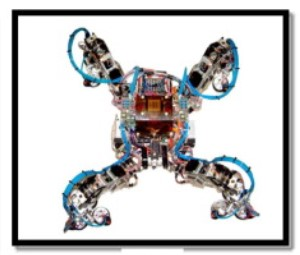
\includegraphics[height=4.5cm]{IMG_07.jpg}
	\caption{Pentium-III}
\end{figure}
\begin{figure}[H]
	\centering
	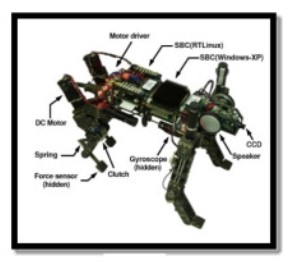
\includegraphics[height=4.5cm]{IMG_06.jpg}
	\caption{AiDAN-I}
\end{figure}
在控制系统实验室,丰田技术研究所展示了一款名为Robocat-1的电动四足机器人,如图15 (a)\supercite{23}所示。在这个机器人中,每条腿有2个总重量为6.85公斤的DOF。这个原型机器人成功地测试了与快速运动控制算法一起使用的小跑循环。
\begin{figure}[H]
	\centering
	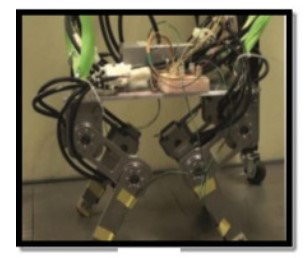
\includegraphics[height=4.5cm]{IMG_08.jpg}
	\caption{Robocat-1}
\end{figure}
\section{国内四足机器人发展摘要}
哈尔滨工业大学开发了一种名为MBBOT的四足机器人\supercite{24},其中所有执行器均由外部液压泵提供动力,如图所示。机器人的每条腿都有四个主动关节,一个被动棱柱弹簧安装在脚部和惯性测量单元(IMU) 中的三分量力传感器。车身总重量为100kg,能够在跑步机上以0.83 m/s的速度跑步。
\begin{figure}[H]
	\centering
	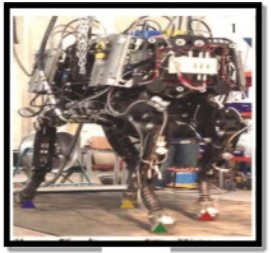
\includegraphics[height=4.5cm]{IMG_11.jpg}
	\caption{MBBOT}
\end{figure}
2013年,上海交通大学研制出一种四足机器人,命名为“小象”,因其外形巨大,能够在各种地形下承载重物,如图11(a)所示\supercite{25}。“小象”由4个串并联混合机构支腿组成,由新开发的液压执行器(Hy-Mo)驱动。

北京理工大学介绍了一种基于液压系统的仿生四足动物原型设计,如图11(b)所示\supercite{26}。该机器人共有16个自由度,由汽油发动机提供动力。机器人可以平稳地进行向后、向前和转弯运动。机器人总重量120公斤,最大前进方向小跑速度3公里/小时。

山东大学2010年开发了一款名为SCalf-1的机器人\supercite{27},如图11(c)所示。该机器人共有12个自由度,一个相同的线性液压伺服缸触发所有执行器。该机器人由IC发动机提供动力,可以以1.8m/s的速度以小跑模式运行。2012年,同一个课题组引进了改进型SCalf-2\supercite{28},在液压动力系统、伺服控制器等方面进行了改造,还安装了惯性测量单元、力传感器等。
\begin{figure}[H]
	\centering
	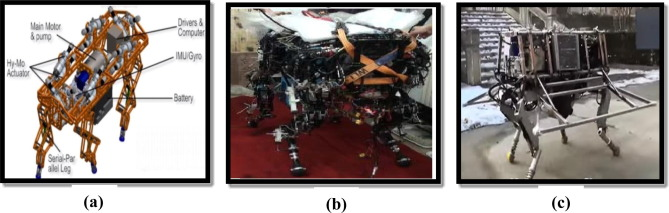
\includegraphics[height=4.5cm]{IMG_10.jpg}
	\caption{国内的机器人}
\end{figure}
\section{现代机器人发展}
2010年,Hutter在苏黎世的瑞士联邦理工学院设计了一只名为Star1ETH的中型犬,如图12所示\supercite{29},该系列高标准弹性执行器安装在star1ETH中,其行为类似于我们的肌腱和肌肉,以暂时保持大量能量。该机器人与IMU结合,IMU提供来自关节​​的运动学信息。另一种多功能四足机器人是为苏黎世 Star1ETH的机器人系统设计的,称为ANYmal,如图12所示\supercite{30}. 它是为石油和天然气平台等具有挑战性的环境中的特殊商业和工业操作而设计的,或者利用其环境感知进行搜索和救援行动。该机器人由高精度执行器驱动,能够实现动态运行步态。小尺寸ANYmal的重量不到 30 公斤,可以携带电池、光学和热像仪、麦克风、动态照明和气体检测传感器等设备。
\begin{figure}[H]
	\centering
	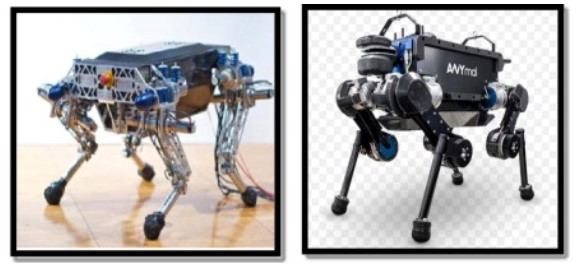
\includegraphics[height=4.5cm]{IMG_12.jpg}
	\caption{star1ETH和ANYmal}
\end{figure}

麻省理工学院于2013年开发了一款名为MIT Cheetah的高效四足机器人\bibitem{31}。研究人员实施了四项设计原则,可以减少运动中的能量损失机制。机器人使用的总功率约为973W,运输成本为0.5,与奔跑的动物非常相似。同一研究所在2015年再次开发了MIT Cheetah-2,如图所示。研究人员成功地在机器人中加入了一种新的算法,以稳定的方式实现了从0到4.5 m/s的范围速度的无束缚运行。该机器人可以在跑步机以及草地和不平坦的地形上以受控方式运行,且可以以2.5m/s的速度跳过高达400mm的障碍。
\begin{figure}[H]
	\centering
	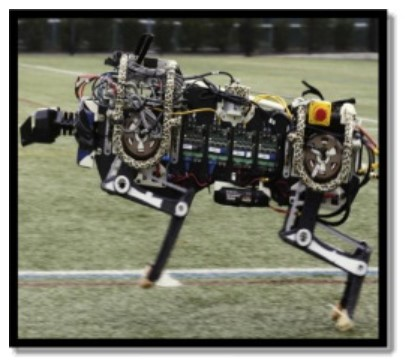
\includegraphics[height=4.5cm]{IMG_09.jpg}
	\caption{MIT Cheetah-2}
\end{figure}
\section{总结及未来方向}
可以看出,先前的机器人领域由国外一家独大,而中国并没有相关的研究,但进入21世纪以后,随着中国科技的发展,机器人领域的研究也开始取得很多不俗的成就,现在中国的机器人在世界上是占有一席之地的。无论是在执行器,步态还是性能等方面,中国研制的机器人有了自己的成就。很明显,过去十年将该领域提升到了一个新的水平,同时为基础和主题开辟了新的研究领域,具有新的机遇。我认为未来的机器人应该包括以下内容:

1.高级机器人不仅需要掌握现有对象,还需要解决现实世界环境中的约束,因此应当尝试将机器人与人工智能等领域相融合,不再将机器人只局限于特定领域的开发与应用,应用人工智能或者机器学习相关领域的内容,让机器人获得更强的适应性。

2.需要对轮足混合动力驱动系统进行更多的研究,使其能够结合两种运动形式的优点,如在崎岖地形中移动和在平坦表面上滚动。

3.将机器人应用到更多的领域上,如医药保健领域,商品分销,协同工作等领域。

\small

\begin{thebibliography}{99}
	\setlength{\parskip}{0pt}

	\bibitem{1} Meng X, Wang S, Cao Z, Zhang L. A review of quadruped robots and environment perception. In: Control Conference (CCC), 2016 35th Chinese. IEEE; 2016. p. 6350–6356.
	\bibitem{2} Y. Zhong, R. Wang, H. Feng, Y. Chen
	Analysis and research of quadruped robot’s legs: a comprehensive review
	Int J Adv Rob Syst, 16 (3) (2019)
	\bibitem{3} Wikipedia. Mobile Robot. Available: https://en. wikipedia.org/wiki/Mobile robot.
	\bibitem{4} P.G. De Santos, E. Garcia, J. Estremera
	Quadrupedal locomotion: an introduction to the control of four-legged robots
	Springer Science and Business Media (2007)
	\bibitem{5} M.H. Raibert
	Legged robots that balance
	MIT Press (1986)
	\bibitem{6} A.C. Hutchinson
	Machines can walk
	Chartered Mech Eng, 11 (1967), pp. 480-484
	\bibitem{7} P.G. De Santos, E. Garcia, J. Estremera
	Quadrupedal locomotion: an introduction to the control of four-legged robots
	Springer Science and Business Media (2007)
	\bibitem{8} S. Hirose, K. Kato
	April). Study on quadruped walking robot in Tokyo institute of technology
	Proceedings of the 2000 IEEE international conference on robotics and automation (2000), pp. 414-419
	\bibitem{9} M.H. Raibert
	Legged robots that balance
	MIT Press (1986)
	\bibitem{10} S. Hirose, K. Kato
	April). Study on quadruped walking robot in Tokyo institute of technology
	Proceedings of the 2000 IEEE international conference on robotics and automation (2000), pp. 414-419
	\bibitem{11} Hirose S, Yoneda K, Tsukagoshi H. TITAN VII: Quadruped walking and manipulating robot on a steep slope. In: 1997 IEEE international conference on robotics and automation, 1997. Proceedings, vol. 1. IEEE; 1997. p. 494–500.
	\bibitem{12} Arikawa K, Hirose S. Development of quadruped walking robot TITAN-VIII. In: Proceedings of the 1996 IEEE/RSJ international conference on intelligent robots and systems' 96, IROS 96, vol. 1. IEEE; 1996. p. 208–14.
	\bibitem{13} Hodoshima R, Doi T, Fukuda Y, Hirose S, Okamoto T, Mori J. Development of TITAN XI: a quadruped walking robot to work on slopes. In: Proceedings. 2004 IEEE/RSJ International Conference on Intelligent Robots and Systems, 2004. (IROS 2004), vol. 1. IEEE; 2004. p. 792–97.
	\bibitem{14} Komatsu H, Ogata M, Hodoshima R, Endo G, Fukushima EF, Hirose S. Development of quadruped walking robot TITAN XII and its basic consideration on the control of large obstacle traversing motion. Trans JSME (in Japanese) 2014; 80(813).
	\bibitem{15} S. Kitano, S. Hirose, A. Horigome, G. Endo
	TITAN-XIII: sprawling-type quadruped robot with ability of fast and energy-efficient walking
	ROBOMECH J, 3 (1) (2016), p. 8
	\bibitem{16} Buehler M, Battaglia R, Cocosco A, Hawker G, Sarkis J, Yamazaki K. SCOUT: A simple quadruped that walks, climbs, and runs. In: Proceedings 1998 IEEE International Conference on Robotics and Automation, 1998, vol. 2. IEEE; 1998. p. 1707–12.
	\bibitem{17} Battaglia RF. Design of the SCOUT II quadruped with preliminary stair-climbing; 2000.
	\bibitem{18} Ingvast J, Ridderström C, Wikander J. The four-legged robot system WARP1 and its capabilities. In: Second Swedish Workshop on Autonomous Systems; 2002.
	\bibitem{19} P.G. De Santos, E. Garcia, J. Estremera
	Quadrupedal locomotion: an introduction to the control of four-legged robots
	Springer Science and Business Media (2007)
	\bibitem{20} Loc VG, Kang TH, Song HS, Choi HR. Gait planning of quadruped walking and climbing robot in convex corner environment 2005; 2005: 314–9.
	\bibitem{21} Koo IM, Trong TD, Kang TH, Vo G, Song YK, Lee, CM, et al. Control of a quadruped walking robot based on biologically inspired approach. In: IEEE/RSJ International Conference on Intelligent robots and systems, 2007. IROS 2007. IEEE; 2007. p. 2969–74.
	\bibitem{22} I.M. Koo, D.T. Tran, Y.H. Lee, H. Moon, J.C. Koo, S. Park, et al.
	Development of a quadruped walking robot AiDIN-III using biologically inspired kinematic analysis
	Int J Control Autom Syst, 11 (6) (2013), pp. 1276-1289
	\bibitem{23} K. Kotaka, B. Ugurlu, M. Kawanishi, T. Narikiyo
	Prototype development and real-time trot-running implementation of a quadruped robot: RoboCat-1
	2013 IEEE International Conference Mechatronics (ICM), IEEE (2013), pp. 604.-609
	\bibitem{24} M. Li, Z. Jiang, P. Wang, L. Sun, S.S. Ge
	Control of a quadruped robot with bionic springy legs in trotting gait
	J Bionic Eng, 11 (2) (2014), pp. 188-198
	\bibitem{25} F. Gao, C. Qi, Q. Sun, X. Chen, X. Tian
	A quadruped robot with parallel mechanism legs
	2014 IEEE International Conference Robotics and Automation (ICRA), IEEE (2014), p. 2566
	\bibitem{26} G. Junyao, D. Xingguang, H. Qiang, L. Huaxin, X. Zhe, L. Yi, et al.
	The research of hydraulic quadruped bionic robot design
	2013 ICME International Conference on Complex Medical Engineering (CME), IEEE (2013), pp. 620-625
	\bibitem{27} X. Rong, Y. Li, J. Ruan, B. Li
	Design and simulation for a hydraulic actuated quadruped robot
	J Mech Sci Technol, 26 (4) (2012), pp. 1171-1177
	\bibitem{28} X. Rong
	Mechanism design and kinematics analysis of a hydraulically actuated quadruped robot SCalf
	Jinan Shandong University (2013), p. 10
	\bibitem{29} Hutter M, Gehring C, Bloesch M, Hoepflinger M, Siegwart R. Walking and running with StarlETH; 2013.
	\bibitem{30} Robotic Systems Lab, ANYmal. Available: http://www.rsl.ethz.ch/robots-media/animal0.html.
	\bibitem{31} D.J. Hyun, S. Seok, J. Lee, S. Kim
	High speed trot-running: implementation of a hierarchical controller using proprioceptive impedance control on the MIT Cheetah
	Int J Robot Res, 33 (11) (2014), pp. 1417-1445

\end{thebibliography}



\end{document}
